%----------------------------------------------------------------------------------------
%	PACKAGES AND OTHER DOCUMENT CONFIGURATIONS
%----------------------------------------------------------------------------------------

\documentclass{article} % Paper and 12pt font size
\usepackage[utf8]{inputenc}
\usepackage[T1]{fontenc}
% \usepackage{libertine}
\usepackage{lmodern} % Use font Latin Modern Sans Typewriter
% \renewcommand{\familydefault}{\ttdefault}
\usepackage[a4paper, margin=1in]{geometry} % Paper size and margin

\usepackage{enumitem} % Format the enumerated list
\usepackage{amsmath,amsfonts,mathtools} % Math packages
\usepackage{amsthm}
\interdisplaylinepenalty=2500
\usepackage{amssymb}
\usepackage[makeroom]{cancel}
\setlength\parindent{0pt} % Removes all indentation from paragraphs - comment this line for an assignment with lots of text

\usepackage{array}
\usepackage{tabu} % Table to text width
\renewcommand{\arraystretch}{1.} % The height of each row in the table is set to 1.5 relative to its default height.
\usepackage[table]{xcolor}

\usepackage{tikz} % Remember picture
\usepackage{graphicx} % Includes images
\graphicspath{ {./images/} } % Tells LATEX that the images are kept in a folder named images under the directory of the main document
\usepackage{wrapfig} % Wrap image i
\usepackage{eso-pic} % used for image background on titlepage
\usepackage{caption}
\usepackage{subcaption}

% Code listing style --------------
\usepackage{listings} % Code listing
\usepackage{color}
\definecolor{codegreen}{rgb}{0,0.6,0}
\definecolor{codegray}{rgb}{0.5,0.5,0.5}
\definecolor{codepurple}{rgb}{0.58,0,0.82}
\definecolor{backcolour}{rgb}{0.95,0.95,0.92}
\lstdefinestyle{mystyle}{
    backgroundcolor=\color{backcolour},
    commentstyle=\color{codegreen},
    basicstyle=\ttfamily\small,
    keywordstyle=\color{magenta},
    numberstyle=\tiny\color{codegray},
    stringstyle=\color{codepurple},
    breakatwhitespace=false,
    breaklines=true,
    captionpos=b,
    keepspaces=true,
    numbers=left,
    numbersep=5pt,
    showspaces=false,
    showstringspaces=false,
    showtabs=false,
    tabsize=2
}
\lstset{style=mystyle}
\usepackage{todonotes}  % Todo



%----------------------------------------------------------------------------------------
%	TITLE SECTION
%----------------------------------------------------------------------------------------
\title{\Huge \textbf{ASSIGNMENT 2} \vspace{.4in} \hrule}

\author{
	\Large ROB521: Mobile Robotics and Perception\\
	\Large Jojo (Yizhi) Zhou, 1003002396\\
}
\date{\normalsize\today}

\linespread{1.3}

\begin{document}
\fontfamily{lmtt} % modern typewriter font

%----------------------------------------------------------------------------------------
%	FRONT MATTER
%----------------------------------------------------------------------------------------
\begin{titlepage}
\tikz[remember picture,overlay]
\node[opacity=1] at (current page.center){
\includegraphics[width=\paperwidth,height=\paperheight]{../Background}};
\vspace*{3.5cm}
{\let\newpage\relax\maketitle}
\vspace*{\fill}

\end{titlepage}

% \newpage
\fontfamily{lmtt} % modern typewriter font

%----------------------------------------------------------------------------------------
%	Q1
%----------------------------------------------------------------------------------------
\section{Occupancy Grid} % The * makes it an unnumbered section

\begin{figure}[hbt]
  \centering
  \begin{subfigure}[b]{0.49\textwidth}
    \centering
    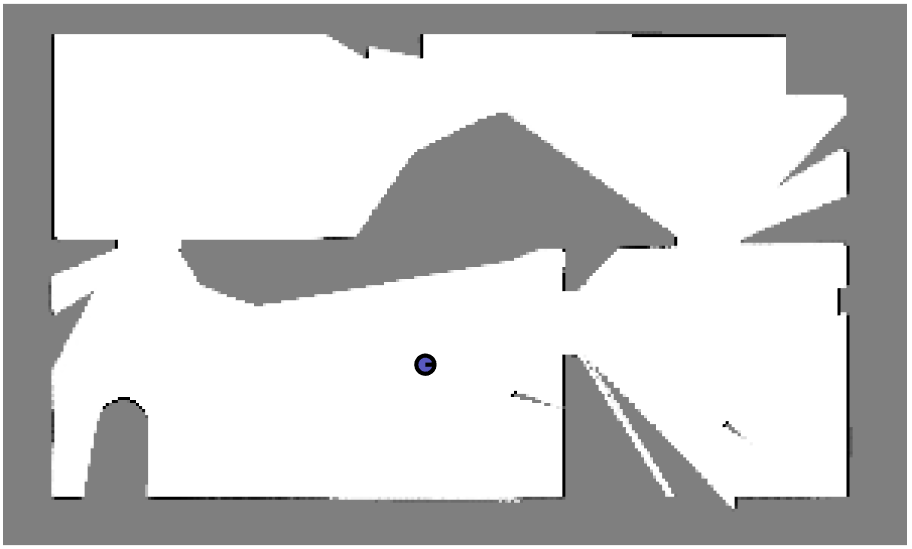
\includegraphics[width=\textwidth]{ass2_q1_a01b1.png}
  \end{subfigure}
  \hfill
  \begin{subfigure}[b]{0.49\textwidth}
    \centering
    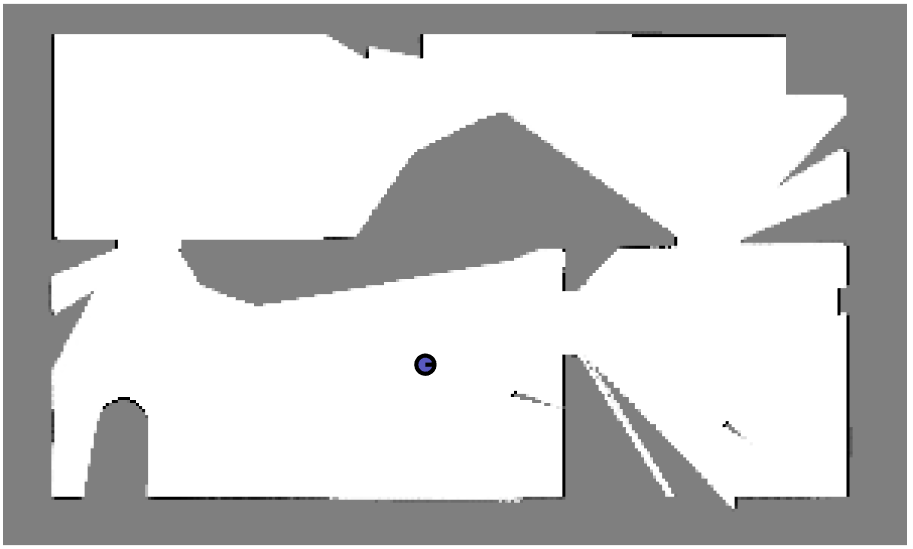
\includegraphics[width=\textwidth]{ass2_q1_a01b1_post.png}
\end{subfigure}
\caption{$\alpha = 0.1, \beta = 1$. Grids updated with absolute value (left) vs. trend (right)}
\label{fig:q1_a1}
\end{figure}

\begin{figure}[hbt]
  \centering
  \begin{subfigure}[b]{0.49\textwidth}
    \centering
    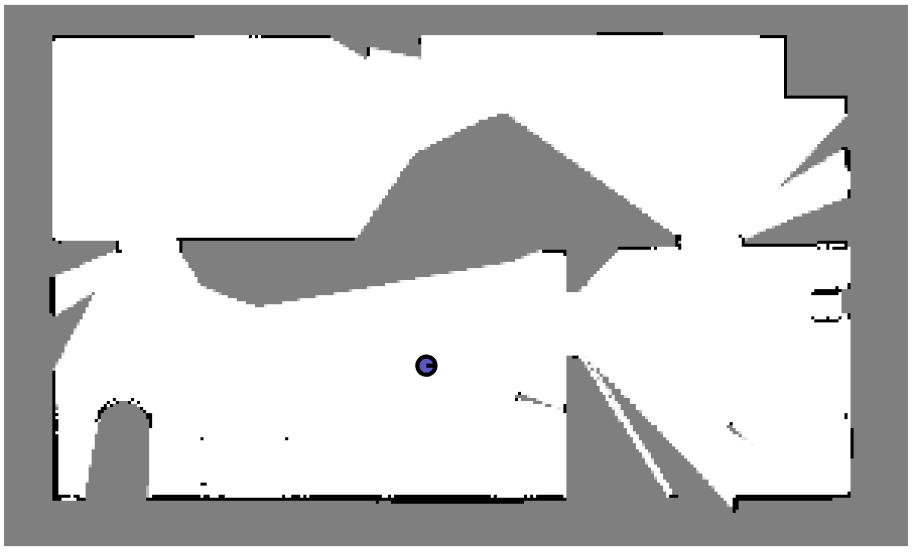
\includegraphics[width=\textwidth]{ass2_q1_a10b1.png}
  \end{subfigure}
  \hfill
  \begin{subfigure}[b]{0.49\textwidth}
    \centering
    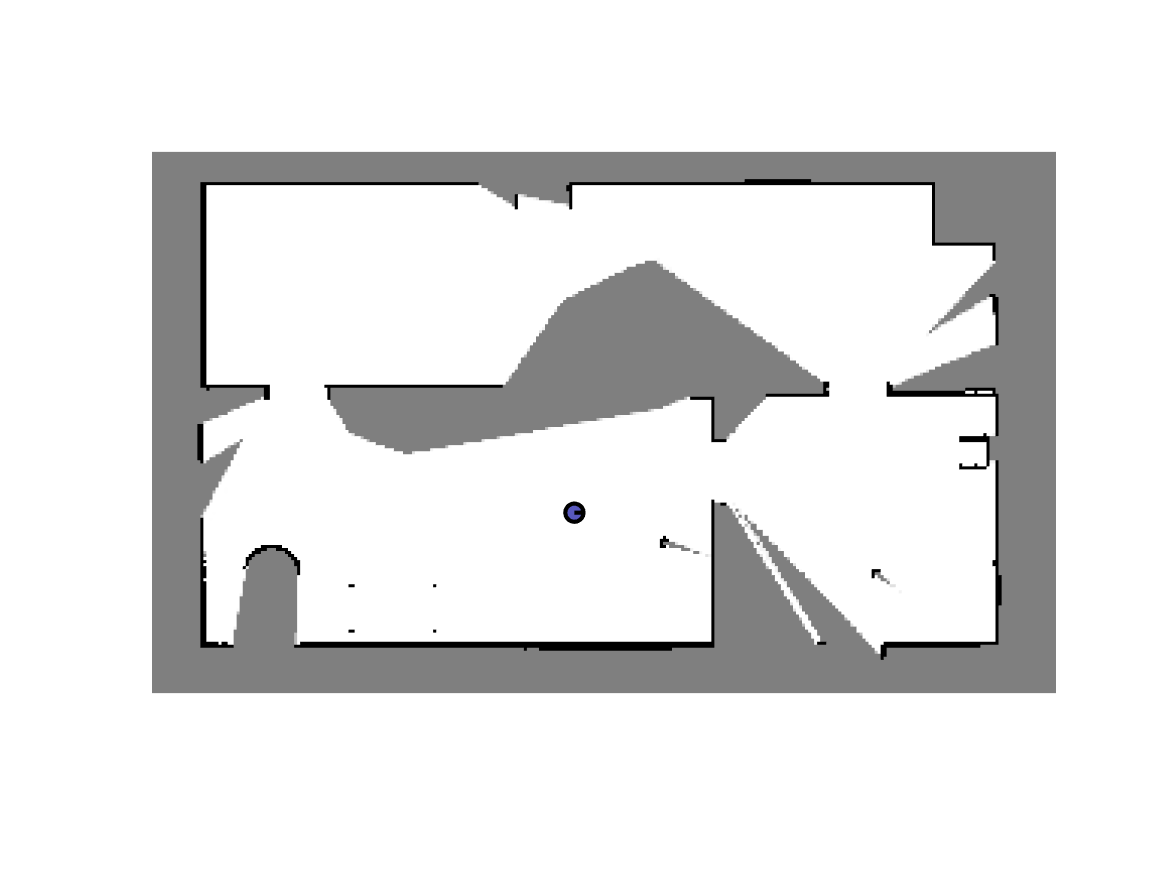
\includegraphics[width=\textwidth]{ass2_q1_a10b1_post_best.png}
  \end{subfigure}
\caption{$\alpha = 10, \beta = 1$. Grids updated with absolute value (left) vs. trend (right)}
\label{fig:q1_a10}
\end{figure}

\begin{figure}[hbt]
  \centering
  \begin{subfigure}[b]{0.49\textwidth}
    \centering
    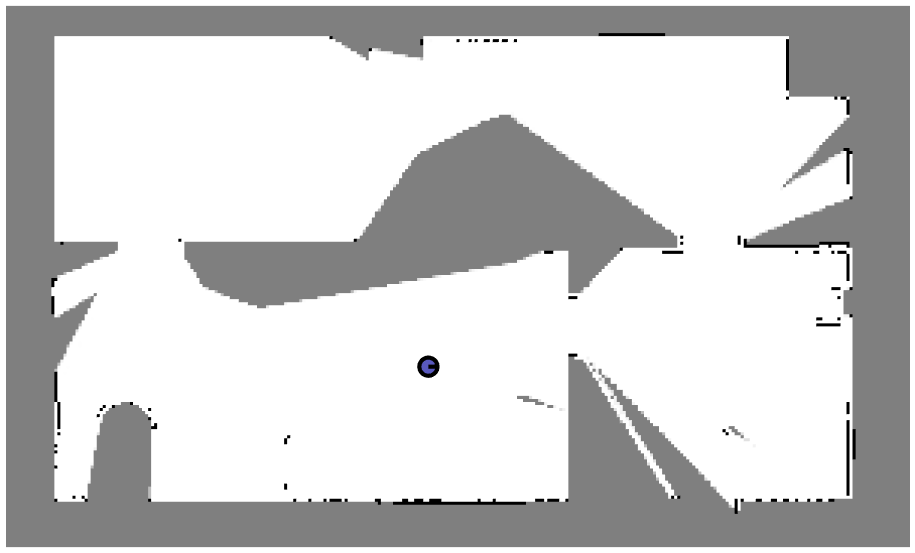
\includegraphics[width=\textwidth]{ass2_q1_a100b1.png}
  \end{subfigure}
  \hfill
  \begin{subfigure}[b]{0.49\textwidth}
    \centering
    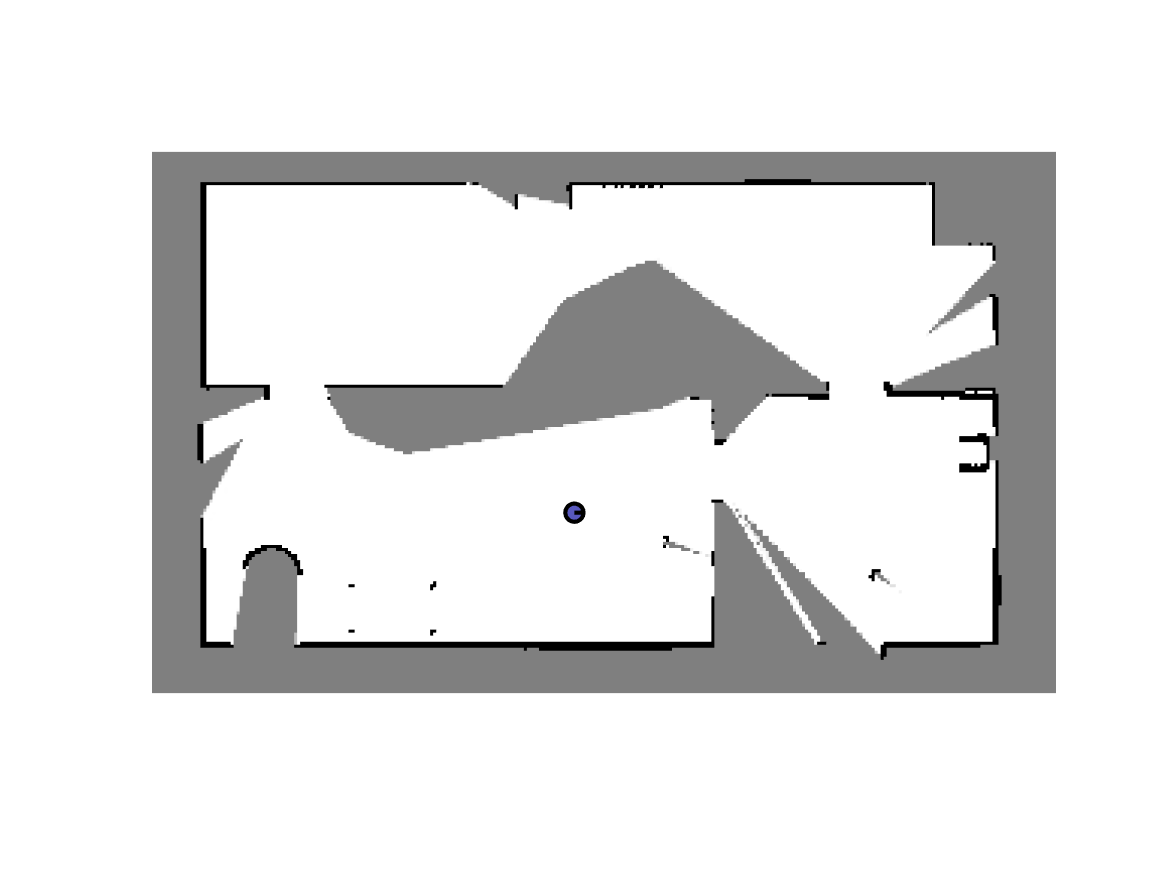
\includegraphics[width=\textwidth]{ass2_q1_a100b1_post.png}
  \end{subfigure}
\caption{$\alpha = 100, \beta = 1$. Grids updated with absolute value (left) vs. trend (right)}
\label{fig:q1_a100}
\end{figure}

The occupancy grids are iteratively updated by the laser scans at each time step. Each laser beam is divided into segments roughly the length of the grids, ranging from the closest to the furthest from the robot:
\begin{itemize}
  \item The furthest laser segment is the obstacle, which blocked the laser beam from reaching further. We add $\alpha$ to the corresponding grid's log-odd value, indicating an increased probability that it is occupied.
  \item Conversely, all the other segments correspond to free space, and we therefore subtract $\beta$ from their log-odd values.
\end{itemize}

While the algorithm is very straightforward, I tuned the $\alpha, \beta$ values and compared the results (fig.\ref{fig:q1_a1}, \ref{fig:q1_a10}, \ref{fig:q1_a100}). We can see that,
\begin{itemize}
  \item In term of $\alpha:\beta$ ratio:
  \begin{itemize}
    \item A smaller $\alpha:\beta$ ratio (fig.\ref{fig:q1_a1}) allows the free-space readings to easily overwrite the previous occupancy reading, resulting in missing walls and obstacles - in fact, the four smaller dots in the bottom-left corner are completely gone.
    \item Conversely, a large $\alpha:\beta$ (fig.\ref{fig:q1_a100}) also results in missing walls, but instead of simply overwriting the probability of occupancy, the behaviour is more inconsistent.
  \end{itemize} 
  \item In term of updating heuristic:
  \begin{itemize}
    \item The left ones update the grid values according to the absolute probability values at each time step, while the right ones' heuristic also requires a tendency. That is, for a grid to be marked occupied, its probability needs to be not only $>50\%$, but also larger than its previous probability (i.e., from the last time step), and vice versa.
    \item We can see, especially from fig.\ref{fig:q1_a10} and \ref{fig:q1_a100}, that using the heuristic with both absolute and relative probability results in a much more consistent result. For example, the walls are less fuzzy.
    \item That being said, the heuristic can't solve the problems from an inappropriate $\alpha:\beta$ ratio (i.e., walls are still missing in fig.\ref{fig:q1_a100}).
  \end{itemize}
\end{itemize} 

I ended up choosing $\alpha:\beta=10:1$ and the heuristic with both absolute probability and tendency, which is shown in fig.\ref{fig:q1}. To further improve the map accuracy, we could simply increase the grid resolution and let the robot explore more, as currently there are apparently some areas that haven't been coved by the laser scans.

\begin{figure}[hbt]
  \centering
    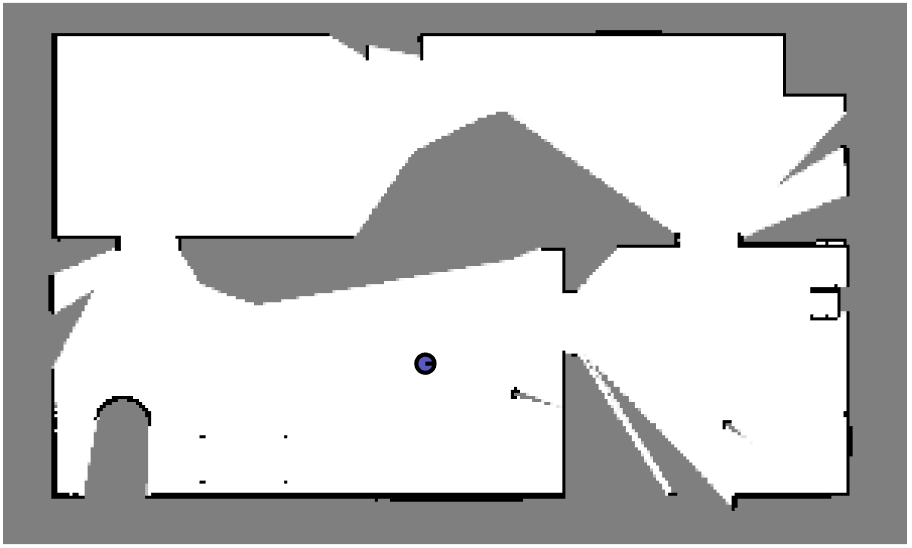
\includegraphics[width=1.0\textwidth]{ass2_q1.png}
  \caption{Final output plot from Question 1}
  \label{fig:q1}
\end{figure}



%----------------------------------------------------------------------------------------
%	Q2
%----------------------------------------------------------------------------------------
\section{Noisy Wheel Odometry}
\begin{figure}[hbt]
  \centering
    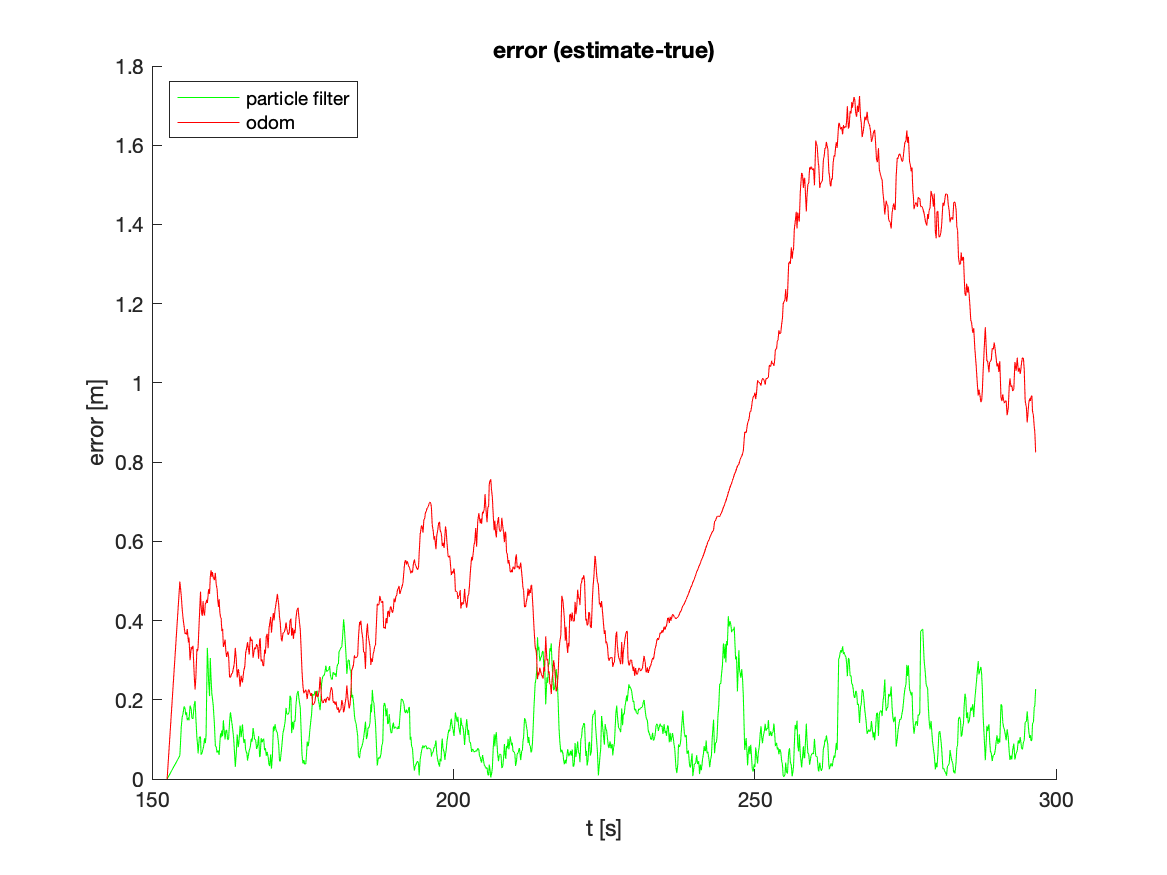
\includegraphics[width=0.9\textwidth]{ass2_q2.png}
  \caption{$\alpha = 10, \beta = 1$ with posterior update}
\end{figure}

In the beginning, the odometry estimate is slightly better the particle filter, as there is little drift in the odometry so far. Near the end of trajectory, the particle filter has trouble estimating the once again, though this time it is significantly lower than the odometry data. This is expected, the divergence of the odometry pose from the true path grows over distance travel.
The growth in error for certain portions likely has to do with the ambiguity of the rooms and the limits of the laser, which caps at 5 meters. With similar features and only a single range value, it is easy for erroneous particles to have high weights. Perhaps with the full 640 angles of laser data, the particle filter will do much better.

The solution error is significantly lower in the beginning and end of the plot; it appears the solution model is more robust to changes in the location compared to my code.
As I am using the same parameters, provided by the model, the main difference should lie in the observation model. I estimated the expected sensor data from the particle using a ray extending from the laser scan pose, incrementally increasing the length of the ray and checking for obstacles.

%----------------------------------------------------------------------------------------
%	Appendix
%----------------------------------------------------------------------------------------
\clearpage
\section*{Appendix I: Code for Occupancy Grid}
\lstinputlisting[language=matlab]{ass2_q1.m}

\clearpage
\section*{Appendix II: Code for Particle Filtering}
\lstinputlisting[language=matlab]{ass2_q2.m}

\end{document}
